\documentstyle[times, graphicx,url,epsfig,alltt,array]{llncs}




\newcommand{\fig}[1]{Figure~\ref{fig:#1}}
\newcommand{\bfig}[1]{(\fig{#1})}

\newcommand{\tbl}[1]{{\fig #1}}
\newcommand{\tion}[1]{\S\ref{sec:#1}}
\newcommand{\btion}[1]{(\tion{#1})}
\newcommand{\stion}[1]{\mbox{(see \tion{#1})}}

\newcommand{\bi}{\begin{itemize}}
\newcommand{\be}{\begin{enumerate}}
\newcommand{\ei}{\end{itemize}}
\newcommand{\ee}{\end{enumerate}}
\newcommand{\bd}{\begin{description}}
\newcommand{\ed}{\end{description}}

\begin{document}

\title{``What is an Agent and Why Should I Care?''}
\author{Tim Menzies\inst{1}, Adrian Pearce\inst{2},
Clinton Heinze\inst{3}, Simon Goss\inst{3}} \institute{ Lane
Department of Computer Science,
        West Virginia University,\\
       PO Box 6109, Morgantown,
       WV, 26506-6109, USA, \protect\url{tim@menzies.com}
       \and
       Department of Computer Science and Software Engineering
The University of Melbourne, \\Victoria, 3010, Australia,
\url{pearce@cs.mu.oz.au} \and Air Operations Division, Aeronautical
\& Maritime Research Laboratory, Melbourne, Australia,
\url{{clinton.heinze|Simon.Goss}@dsto.defence.gov.au}}

\pagestyle{plain} \thispagestyle{plain} \maketitle

\begin{abstract}
A range of agent implementation technologies are reviewed
according to five user-based criteria and via a comparison with
object-oriented programming. The comparison with OO shows that
some parts of object technology are a candidate implementation
technique for some parts of agent systems. However, many other
non-object-based implementation techniques may be just as useful.
Also, for agents with mentalistic attitudes, the high-level
specification of agent behavior requires numerous concepts outside
the object paradigm; e.g. plans, communication, intentions, roles,
and teams.

KEYWORDS: evaluation, agent-oriented, object-oriented.
\end{abstract}

\section{Introduction}

Is there anything really new in agent-oriented software? Are agents a
bold step forward into the future of software? Or is agency just
``new wine in old bottles''?

Our users demand answers to these questions, and others. One
 gruff user always asked ``what are agents and
{\em why should I care}?''. To such users, the issue in italics is
the key question. Agent technologies are interesting to users {\em
only} if those technologies address issues of interest to the
users.

After explaining agents to this gruff user, this users next
comment was ``this sounds just like OO to me; what's new here?''.
Such comments motivate this article. Our response to these
comments is in three parts: \be \item We carefully define the core
concepts of agent-oriented software and object-oriented software.
\item Next, we review the diverse range of software labelled
``agents''. \item This software is then assessed these concepts
with respect to certain user-oriented issues. \ee
\begin{figure}[!t]
{
\begin{center}
\begin{tabular}{r@{ : }p{2.7in}|c}
{\em Name} & {\em Notes} & {\em Introduced in...}\\\hline
 OO & Object-oriented &
\tion{wa}
\\\hline Standard BDI & BDI= beliefs, desires, intentions
&\tion{bdi}
\\\hline
 FORTRAN & How we used to build agents & \tion{mod} \\\hline
 dMARS & A commercial agent-oriented BDI tool & \tion{mod}
\\\hline
Command agents & Heinze and Pearce's extension to dMARS &
\tion{ca}\\\hline Behavioural cloning & Machine learning to build
agents & \tion{clone}\\\hline Petri nets & & \tion{rely} \\\hline

TACAIR/ SOAR/ PSCM & The problem space computational model (PSCM)
is how the rule-based system called SOAR implements TACAIR, an
agent system. & \tion{kb} \\\hline

G2 & Gensym's rule-based expert system shell: includes powerful
interface tools. &\tion{xplain}
\\\hline MBD-based & The model-based diagnosis system used in
NASA's remote agent experiment (RAX). & \tion{speed}
\\
\end{tabular}
\end{center}
} \caption{Agent implementation technologies discussed in this
article}\label{fig:sys}
\end{figure}

The user issues used in this article come   from the Australian
Workshops on Agent-Based systems. Those workshops have debated the
relative merits of the agent implementation technologies shown in
\fig{sys}. In those debates, the technologies were assessed with
respect to the problem of building agents for the  Air Operations
Division (AOD) of the Australian Defense Science Technology
Division.

For several years, the Australian Defense Forces have been using
agent-oriented software to assess potential new hardware
purchases.  Buying planes and helicopters for the Air Force
implies a major commitment to a particular platform.   AOD uses
operational simulation for answering specific questions about very
expensive equipment requisitions, component capabilities and
rehearsing dangerous tactical operations.   In pilot-in-the-loop
flight simulation, intelligent pilots (agents) interact with each
other in the computer simulation, as well as the human pilot in
the virtual environment. These dynamic, interactive multi-agent
simulations pose a challenge for the integration of valid pilot
competencies into computer controlled agents. This involves
modeling pilot perception through recognition of actions and
events that occur during simulation. Such simulators are often
used after purchase as training tools. Hence, a core task within
DSTO is the construction and maintenance of agent-oriented
systems. These AOD agent simulations push the state-of-the-art:
\bi \item AOD agents interact at high frequency in a dynamic
environment  with numerous friendly and hostile agents. For
example, AOD agents engage in complex aerial maneuvers against
hostile high-speed aircraft. \item AOD agents co-ordinate
extensively to achieve shared goals. For example, a squadron of
fighters may collaborate to shepherd a cargo ship through enemy
lines. \item AOD agents may change their roles at runtime. For
example, if the lead of a fighter formation is shot down, then the
wing-man may assume the role of fighter lead. As roles change,
agents must dramatically alter their plans. \ei

After discussions with AOD users, the following concerns were
identified. These concerns are the basis for our user-oriented
discussion  of the merits of different agent technologies:  \bi
\item Easy of construction/ modification. \item Provable
reliability. \item Execution speed. \item Easy of explanation of
agent behaviour. \item Support for {\em teaming}. Teaming is a
special AOD requirement which is described below and may not be
widely relevant. \ei


The rest of this article debates the merits of the agent
implementation technologies of \fig{sys} for AOD applications.
After that debate, we will see that agent-oriented systems
requires much that does not exist in standard software engineering
methods: \bi \item
 AOD agent programmers do not spend their time
fretting about encapsulation, classification, etc. \item
 Instead,
they concern themselves with concepts such as plans,
communication, perception, intentions, roles, and teams. \ei
This
is not to say that standard methods such as (e.g.) object-oriented
are irrelevant to agent construction. At the end of this article
we will briefly describe how objects are used within AOD agents
for building environments in which we specify agent behavior.



\section{Agents Versus
Objects}

Before proceedings,   we digress for a brief introduction to agents. In order
to simplify the reader's introduction to agents, we will stress the
similarities and differences of agent technology to object technology. In what
the literature calls  {\em  weak agents} maps neatly into object technology.
However, object technology is incomplete for implementing what the literature
calls {\em strong agents}.



\subsection{Weak Agency}\label{sec:wa}

A spectrum of agents types is  offered by Woolridge and
Jennings~\cite{woolridge95}. Within that spectrum we say that AOD's agents are
at least {\em weak agents} since they are {\em autonomous, social, reactive}
and {\em proactive}. They are {\em autonomous} since, while the  simulations
execute, AOD  agents act within intervention by a human operator.  They are are
also {\em social} in the sense that  AOD's agents interact extensively with
other agents. Also they are  {\em reactive} since AOD analysts develop
different scenarios for their agents. Within each scenario, AOD's agents must
react to changing circumstances. Further, they are {\em proactive} since AOD
agents can take the initiative within a simulation.

Woolridge and Jennings comment that concurrent object-oriented languages
provide much support for weak agents.   According to the UML community (e.g.
Booch~\cite{booch94}), OO technology consists of at least {\em identity, state,
behavior, classification, inheritance, polymorphism} and {\em encapsulation}.
These terms, and there relations to agents, are described below.

 An object is
something that can be clearly distinguished from other concepts in the design.
Agents can use this {\em identity} to distinguish themselves from other agents.

 Objects are repositories of  data. Synonyms for
this {\em state} include attributes or data.

 Objects are also
repositories of  pre-defined {\em behaviour}. Synonyms for behaviour include
methods, functions, procedures, or code. Agents can use state and behaviour to
model their beliefs and actions on the world. Further, identity-specific
behaviour lets us implement agent {\em pro-activeness}; each agent-object can
carry with itself an agenda of tasks to be performed.

Each object can be categorized into exactly one class. This {\em
classification} defines the state and behaviour that is valid for that object.
Agents can use classification to simplify  their reasoning about other objects
in the domain. For example, if an agent recognizes that the object {\tt
LauraBush} belongs to the {\tt Person} class, then they can access default
knowledge about {\tt LauraBush} from {\tt Person}.

Objects can be defined via extensions to parent objects. Services and
invariants of such parent objects can be relied on within all the parent's
children since parent properties are {\em inherited}. Agents can use
classification to simplify their own internal implementation as well as
extending their classification knowledge.

 Behaviors can
be implemented in different objects using the same name. This {\em
polymorphism} implies some kind of message-passing system; i.e. the results of
a particular message is computed from the name of message and the nature of the
receiver of that message. The same message sent polymorphically to different
objects may generate different responses. Agents can use polymorphism to  group
together the services offered by other agents. For example, an agent might
assume that all other agents in their domain respond to messages such as
"position" or "velocity". Polymorphism means agents can assume simple and
common interfaces to other agents; i.e. polymorphism simplifies the
implementation of  agent {\em social ability}.

 Clients of an
object should not need access to the internal details of that object. Such
clients can ask an object to perform a named service without needing to know
the details of how such services are implemented. Agents can use this {\em
encapsulation} to ensure that, when they run {\em autonomous}ly and
asynchronously, their internal knowledge is not mixed up with the knowledge of
other agents.



\subsection{Strong Agency}\label{sec:bdi}

According to Wooldridge and Jennings, {\em strong agents} may possess
mentalistic attitudes or be emotional or animated. AOD agents lack emotion but
are mentalistic. AOD agents are based on the {\em beliefs}, {\em desires} and
{\em intentions} (BDI) paradigm of~\cite{rao95}. The current state of entities
and environment as perceived by the agent (abstract labels or percepts) are the
agent's {\em beliefs}. A {\em desire} is some  future states agent would like
to be in (a.k.a. goals). {\em Intentions} are some  commitment of an agent to
achieve a goal by progressing along a particular future path that lead to the
goal (a.k.a. a plan). One advantage with using intentions is that the effort
associated with creating them need not be repeated every time they are
required. Intentions can be pre-computed and cached. Each intention can be
tagged with a trigger describing some situation in which this intention should
be accessed and applied.

In this BDI paradigm, deliberation is done through the selection
of a goal, selection of a plan that will be used to form an
intention, selection of an intention, and execution of the
selected intention. All these decisions are based on the beliefs
the agent has about the current state of the environment. The
process of selecting the forming plan is known as means-end
reasoning.



The BDI means-end reasoning approach has proven very beneficial to
the AOD, particularly the OPERATOR AGENT that is used to simulate
military operations, it is used in support of multi-billion dollar
requisitions~\cite{tidhar99}. This is partly reflected in the
maturity of BDI, and the fundamental limitations it
overcomes~\cite{rao95}. This includes ways of relaxing the need to
have perfect knowledge of opponents' plans.

The BDI approach has made it easier for DSTO to codify tactics and
build simulations, and importantly, to get explanations out of
them of what happens. The DSTO has found it easier to construct
and modifying scenarios, as the Operator Agent is a generalized
agent capable of simulating different entities, aircraft, ships
etc. Implemented using the dMARS procedural reasoning
language~\cite{dinv98}), BDI improves abstraction for
representation of declarative and procedural knowledge. This
allows for improved explanation, as the success of these
operational simulations is measured in terms of what all
stakeholders receive, whether experts or operators.

The BDI approach has also scaled up for large scale operational
simulation-the Operator Agent at the Air Operations Division (AOD)
has been used to run operational simulations involving 32 pilots,
400 plans, 10 goals, 25 intentions concurrently, each receiving 8
contacts every 50ms~\cite{tidhar99}.

\begin{figure}[!t]
\begin{center}
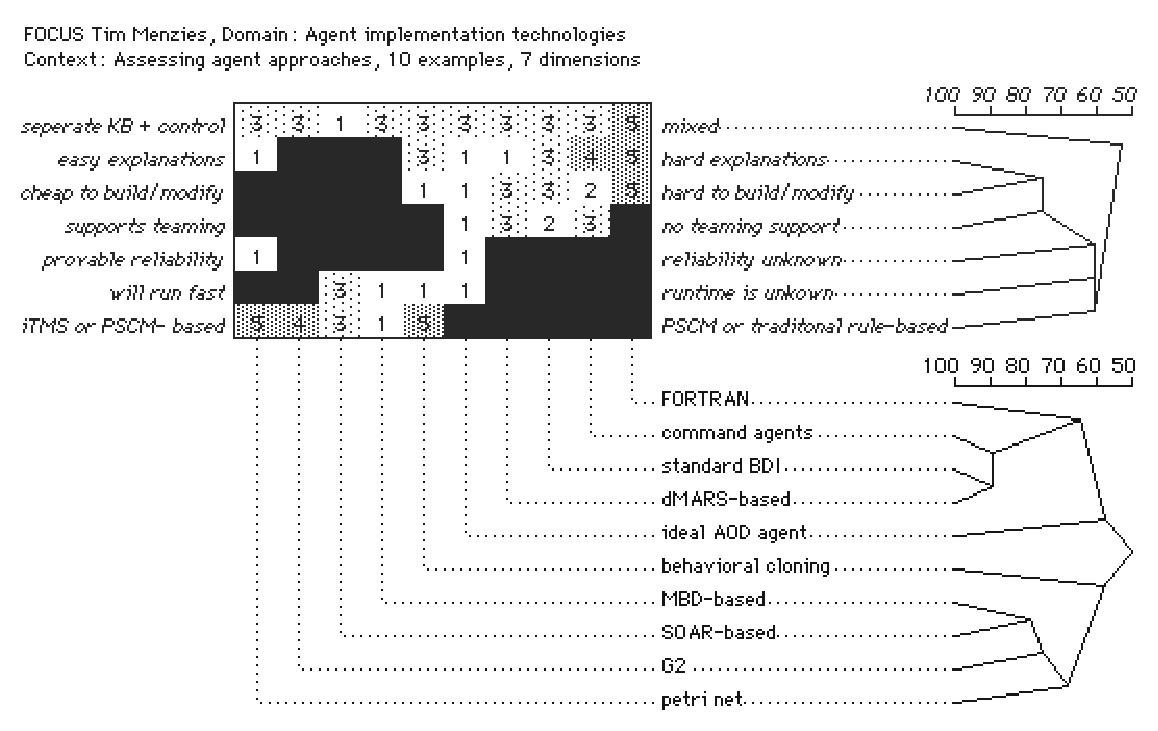
\includegraphics[width=5in]{table.eps}
{\em  {\sffamily
\begin{quote}
A repertory grid maps {\em examples} into a range of {\em dimensions}. For any
row in the table, if an example scores "5", it is near the right-hand end of a
dimension. If it scores "1", it is near the left-hand end of a dimension. For
example, bottom left, petri nets scores a "5"; i.e. it is more a rule-based
system than a iTMS or PSCM-based system. Black areas denote ``don't know''.
Trees on far right show distances between each example and dimension; e.g.
standard BDI and dMARS-based systems are very similar.

\end{quote}
}}
\end{center}
\caption{A comparison of implementation issues for agents.
Generated from the web-based repertory grid server at
\protect\url{http://gigi.cpsc.ucalgary.ca/}.
 }\label{fig:table}
\end{figure}



\section{A Range of Agent Technologies}

In this section, we explore a range of  agent implementation
technologies considered at AOD. All our implementation options are
compared to some mythical ideal AOD agent system  in the {\em
repertory grid} of \fig{table}. \fig{table} shows various
implementation options (e.g. G2) ranked on different dimensions
(e.g. easy/hard to modify).  Repertory grids are a knowledge
acquisition technique extensively explored by Shaw and
Gaines~\cite{shaw97,gaines89}. Their key benefit is that
superfluous  comparisons between examples are ignored. Dimensions
are only added to a repertory grid if they help to distinguish
examples. That is, dimensions with no information content are
excluded. A side-effect of this approach will be that we will not
define in detail different agent implementation technologies.
Instead, we will just discuss how these technologies differ
according the repertory grid dimensions.  However, we do provide
references for each method so the interested reader can explore
further.

The rest of this section defines the dimensions of \fig{table}.
The desired end of each dimensions will be shown as headings while
the opposite, and undesirable, end of each dimension will be shown
in italics.



\subsection{Easy to Build/Modify}\label{sec:mod}

{\em Opposite= hard to build/modify.}

AOD's agents are used to handle specialized what-if queries.
What-if queries are notoriously ad hoc. Ideally, we should be able
to quickly change our agents to accommodate new what-if queries.

Originally, AOD ran its agent simulations using standard
procedural languages to implement the decision logic of a human
operator. In procedural systems (e.g. FORTRAN) such decision logic
may comprise less than 20\% of the total system. However, such
code can consume up to 80\% of the maintenance effort. For
example, new programmers working on a FORTRAN  simulator could
take up to one year before be able to modify the decision logic.

In response to this maintenance cost, AOD turned to high-leval
BDI-based agent-oriented languages. Agent-oriented software such
as dMARS~\cite{dinv98} offers a succinct and high-level
representation of the decision logic. Using such agents, AOD has
been very successful in reacting to customer "what if" queries
from their customers. With the FORTRAN systems, in might have
taken weeks before AOD could report simulation results from
different operator actions. With the agent systems, such reports
can be generated in days or even hours.

Standard BDI is a conceptual framework that must be supported by a tool such as
dMARS in order to be practical for real-world practioners.  dMARS offers
high-level  support for BDI and extensive graphical facilities. dMARS reduced
the cost of creating AOD agents. However, even though costs were significantly
reduced, AOD still finds agent design to be very expensive. Two technologies
that address the cost issue are {\em command agents} and {\em behavioral
cloning of agents}, discussed below.

\subsubsection{Command
Agents}\label{sec:ca}

Pearce and Heinze  added another layer on top of dMARS to process the patterns
of standard agent usage seen at AOD~\cite{pearce00,heinze02}. Their {\em
command agents} divide reasoning into the following . Firstly, {\em  situation
awareness} extracts the essential features from the environment. Next, the {\em
 assessment} layer ranks the extracted features. These ranking represents a
 space of options explored by {\em
  tactic selection:}. lastly, in the
{\em selection of operational procedure} layer, the preferred option is mapped
  onto the available resources.


In repeated applications of this framework, Pearce and Heinze
report that the command agents framework offers  a significant
productivity increase for AOD personnel over standard dMARS.

\subsubsection{Behavioral Cloning of
Agents}\label{sec:clone}

{\em Behavioral cloning} is a machine learning technique. A
qualitative model of a domain is generated. The qualitative model
is imprecise and so contains areas of uncertainty.  A scenario is
described. This scenario serves to restrict the ranges of some of
the uncertain values within the model. The model is now executed
within the constraints offered by the scenario. Where uncertainty
exists, the simulator either picks one option at random or
backtracks over all options (if such backtracking is tractable).
This simulation generates an experience base: a file of examples
of the operation of the model. The experience base is then
classified according to some domain criteria; e.g. we never ran
low on fuel. A machine learner then generates some summary of the
classified examples. This technique has been used to generate
knowledge of cardiac function~\cite{bratko89},  satellite
electrical systems~\cite{pearce88}, how to fly a
plan~\cite{sammut92}, and how to run a software
project~\cite{me00a}.

Behavioral cloning often throws the   intermediaries between
inputs and outputs. Hence, a disadvantage of behavioral cloning is
that the learnt theory can't queried for a rich description for
{\em how} some output was reached. Hence, behavioral clones may be
hard to explain.

On the other hand,   behavioral cloning scores highly on the
``easy to build/modify'' scale. Once the background qualitative
model has been built, the knowledge required for a new agent can
be generated automatically merely by adopting new scenario
constraints.

\subsubsection{Easy to Modify: Summary}

Clearly FORTRAN scores the lowest on this dimension and behavioral cloning,
theoretically anyway, scores the highest. dMARS is mid-range on this scale and
command agents are easier to modify than standard dMARS systems.

\subsection{Supports Teaming}

{\em Opposite= no teaming support}

Teams  are a natural means of modeling collaborating defense
forces. Teams act as if they share a belief set even though
sometimes team members may have subtlety different beliefs. While
team member A may not know everything known by team member B, some
abstract co-ordination agent knows everything that the team
members know.

The current generation of agent software used at AOD is designed
for modeling the interaction of solo agents in a shared
environment. Coding such tools gets complex when teams co-ordinate
and share beliefs. In particular, every exception case where the
team believes X while the team member believes Y must be encoded.

At present, AOD makes little use of team-based agent simulations:
i.e. most of its systems are at the first-person singular level.
Consequently, the spaghetti sections are not large. However,  it
is anticipated that in the near future, AOD will be making
extensive use of team-based simulations.

Some initial experiments have been performed with implementing
teaming in a dMARS framework~\cite{tidhar98}. These initial
studies may also supply command agents with a teaming ability
(since command agents are  built on top of dMARS). Apart from
that, the AOD experience is that most agent systems have very
little support for teaming.

\subsection{Provable reliability}\label{sec:rely}

{\em Opposite= reliability unknown.}

Currently, AOD's agents are only used in the research labs.
However, this may change. Each simulator stores extensive tactical
knowledge that could be usefully applied in the field. However,
before a research prototype can be deployed into the field, its
reliability must be certified. In the context of this article we
say that reliability is some probability that, after watching the
system run and seeing some errors, that in for future time $T$ we
will see $N$ errors.

Within AOD there has been some discussions on using petri nets to implement
agents. A petri net~\cite{reisig82} is a directed graph interconnecting nodes
of different types on which multiple tokens are permitted to travel. There are
two types of nodes: places and transitions. Arcs connect places to transitions
and transitions to places; transitions are never connected to transitions, and
places are never connected to places. While Petri nets consist of a small
number of elements and the algorithms for evaluation can be expressed very
simply, they are sufficiently formal to allow mathematical analysis. These tend
to be both detailed and complex. A large suite of reliability results exist for
petri nets (as used in Markov chains~\cite[p759-765]{lyu96}) or
otherwise~\cite{kummer00}. Agents based on petri-nets/markov models have been
used in domains as complicated as Robocup\cite{han99} (though Pearce, Heinze
and Goss comment that such single state systems do not adapt well when there
are multiple entities operating in the simulation~\cite{pearce00,heinze02}).


Petri nets are a convenient tool for reasoning about concurrent
systems.  Unlike a state transition diagram, where execution is
sequential, traversing one state after another, with petri nets
execution is fully concurrent. Hence, it has been argued that
petri nets are a sound basis for constructing reliable agents.

On balance, it is doubtful that AOD will adpot the petri net
approach, due to the next point.

\subsection{Separate KB and Control}\label{sec:kb}

{\em Opposite= Mixed.}

AOD has a strong commitment to cognitive modeling; i.e.
generating
human-like behaviour from explicit high-level symbolic
representations. Hence, an ideal AOD agent uses such
representations.

Different approaches to agent-based systems take a different
approach to their representations. General BDI is a conceptual
framework, not a specific implementation. Hence, it makes no
commitment to levels of control flexibility. Procedural languages
like FORTRAN mix domain knowledge and inference knowledge like
spaghetti. Recall that it was the maintenance effort associated
with such spaghetti code that drove AOD away from FORTRAN.
Knowledge based systems take a separate approach: inference and
domain knowledge are distinct and can be modified separately. All
the non-FORTRAN agent systems being discussed here can be divided
up according to how flexible is their control knowledge.

At one end of the control flexibility-scale are agents based on
the SOAR architecture (e.g. TACAIR~\cite{jones99}). A SOAR
knowledge base has two distinct parts: a standard declarative rule
section and a second section describing the control knowledge in
rule-based terms. In SOAR, agents seek operators which might take
them closer to their goals. Conflict resolution  is used to
resolve conflicts between competing operators.  Conflict
resolution is SOAR,  the operators, and the domain rule knowledge
are all implemented in the same uniform rule-based manner.  This
means that the knowledge engineer can customize not only the rule
base but also the control of how the rules are fired. Rules in
SOAR are organized into problem spaces: zones within the kb that
discuss the same sets of operators. If a SOAR problem space can't
resolve operator clashes, then a {\em impasse} is declared and
SOAR forks a nested problem space with the task of resolving that
conflict. Hence, at runtime, a SOAR system conducts a recursive
descent through the problem spaces. This is called the problem
space computation model (or PSCM~\cite{yost89}).  Recursive
descent is only an approximation of PSCM. Each problem space is an
autonomous group of rules that  might "wake-up" and execute if
their pre-conditions are ever satisfied. The authors of TACAIR use
this feature extensively. TACAIR views its knowledge as an
intricate goal hierarchy.  Problems spaces act like min-agents;
each with their own autonomous agenda that sleep till some trigger
condition makes them execute.

At the other end of the control flexibility-scale are petri nets
and the decision trees generated by behavioral cloning. Petri nets
and decision trees permit no meta-level control of the inference
net. In marked contrast to SOAR, inference is via inflexible local
propagation rules. It would be a simple matter to add a
meta-interpreter to (e.g.) petri nets that could customize the
propagation rules. However, such meta-level control would change
the runtime properties of a petri net and invalidate all the petri
net reliability results.

Halfway between the total flexibility of SOAR and the rigid
inflexibility of petri nets/decision trees lies the BDI support
systems ( dMARS, command agents). These system restrict the
knowledge engineer into creating planning systems. However, within
that restriction, considerable flexibility is offered.

\subsection{Easy explanations}\label{sec:xplain}

{\em Opposite= hard explanations}

Defense personnel  audit AOD agent knowledge bases to see if they
reflects current Australian defense tactical maneuvers. Hence, it
is important that the inner workings of agents can be explained to
a domain expert.

Explaining the behaviour of a agent generated from behavioral
cloning is difficult. The learnt theory is a mapping of inputs to
outputs with all internal connections thrown away. Such internal
connections are useful in building rich explanation structures.
Still,  the simplicity of the decision tree generated from
behavioral cloning makes cloned agents easier to understand than
those written in some procedural language (e.g. FORTRAN).

AOD supports at least two methods for generating intricate
explanations. Firstly, they claim that the agents knowledge base
is close in concept to how human operators control defense
hardware. At AOD, agency is not merely some implementation trick.
Rather, by explicating agent knowledge, AOD is hoping that it is
also explicating  human knowledge at a comprehensible level of
abstraction. Further, the command agents paradigm sits well with
standard operational practice within the Australian defense
forces. Hence, AOD argues, explaining an BDI/command agents tool
is fundamentally simpler than browsing some other conceptual model
(e.g. FORTRAN code).

Secondly, AOD uses explanations via graphical visualizations. The
dMARS tool makes extensive use of graphical interfaces. Another
implementation tool of note is the G2 system. Clancey {\em et.al}
have used G2 to build elaborate agent systems in which the
behaviour of an organization is emergent from the behaviour of the
agents representing the workers in that
environment~\cite{Clancey96a}. G2 offers extensive support for a
traditional rule-based execution paradigm. G2 is also a powerful
tool for building elaborate graphical interfaces (e.g.~\fig{g2}).

\begin{figure}[!h]
\centerline{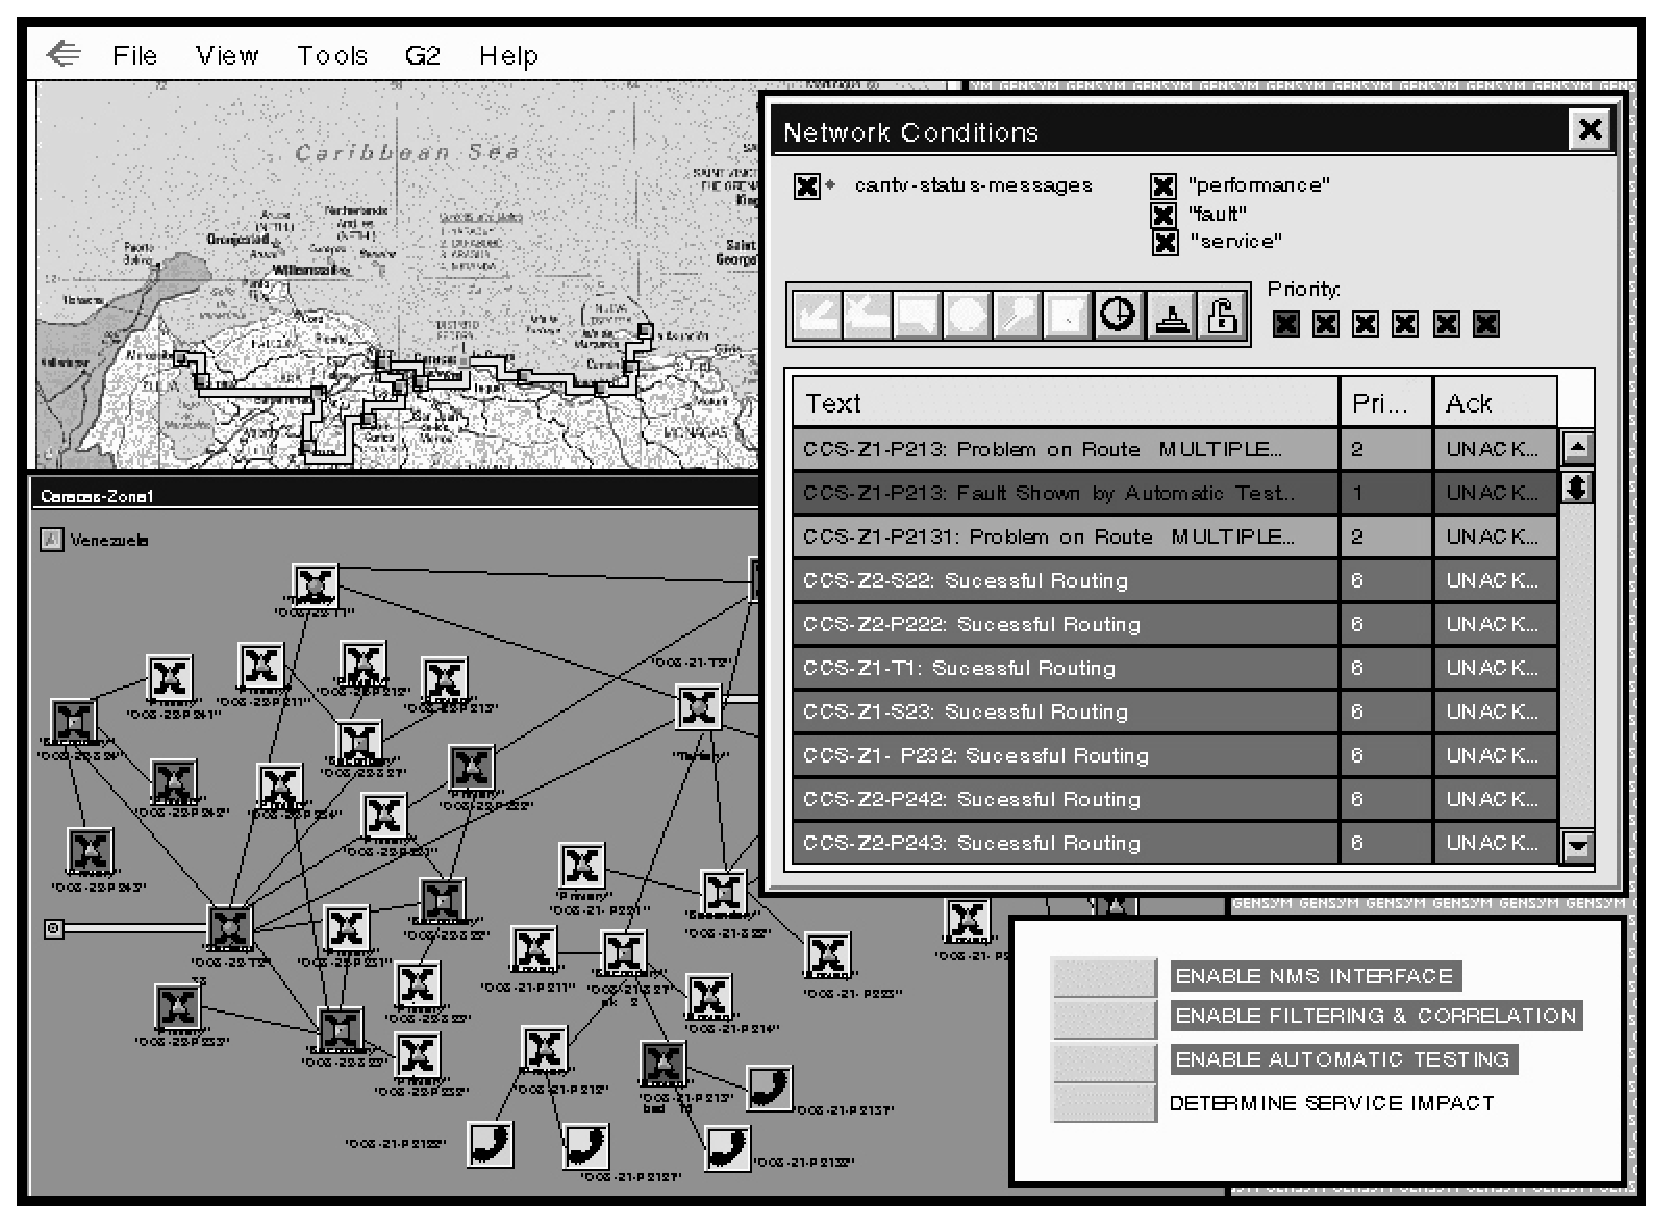
\includegraphics[width=4.5in]{g2.eps}} \caption{Sample screensap
from a G2 application. From\newline
\protect\url{http://www.gensym.com/products/operationsexpert.htm}.}\label{fig:g2}
\end{figure}

\subsection{Tractability/speed results known}\label{sec:speed}

{\em Opposite= tractability/ speed is an open issue}.

Repeating the above point on reliability, if a research prototype
is to be deployed into the field, we need some assurance that it
will execute at least as fast as events in the field.

Behavioral cloning builds decisions trees and such trees execute
very quickly at runtime. While this is a significant advantage of
behavioral cloning, we note that this comes at the cost of all the
disadvantages mentioned above; e.g. poor explanatory capacity.

In terms of reasoning efficiency, an interesting middle ground
between decision trees and BDI is the agent technology used by
NASA in its remote agent experiment (RAX). NASA deployed RAX in
the asteroid belt in May 1999. RAX  built its own autonomous plans
to react to flight events~\cite{musc98}. The representations
within RAX were much simpler than (e.g.) the AOD BDI plans. The
RAX development team claim that, after several years with
exploring model-based diagnosis (MBD), that very simple
representations can model even complex domains. Further, given
regular propositional encodings of that domain knowledge, an
incremental truth maintenance system (iTMS)~\cite{pand97} can
build satisfactory plans very quickly.


\section{Conclusion}

The goal of this paper was to assess agent-oriented systems via
two kinds of user-oriented queries. Firstly, our users were
worried about the (non)-distinction between agents and objects. As
seen above, the ``OO mindset'' contains about half a dozen key
concepts: class, instance, encapsulation, inheritance,
polymorphism, and so on. However, the key concepts of  the AOD
``agent-oriented'' mindset make little reference to the key OO
concepts. For example, OO makes no reference to the concept that
AOD regards as central to agency: intentionality. Nor do the core
OO concepts refer to explicit knowledge representation of domain
and control knowledge, teaming, plans, communication, perception,
beliefs, and desires.   Further, the assessment criteria we would
apply to agent systems are orthogonal to the key OO concepts  and
include ease of construction and maintenance, ability to explain
agent knowledge, and promises of runtime performance, reliability.



Secondly, our users were concerned about the range of issues and
the range of technologies clustered in  \fig{cluster}.  This
figure is a 2-D display of a n-dimensional space and so cannot be
a totally accurate representation. However, it does clearly show
the distance of FORTRAN to AOD's ideal agent technology. Further,
the low-level representations of petri nets and the MBD-based RAX
system make them poles apart from AOD's ideal agent. Behavioral
cloning is surprisingly close to AOD's ideal; perhaps only because
of its ease of construction.


\begin{figure}[!t]
\begin{center}
 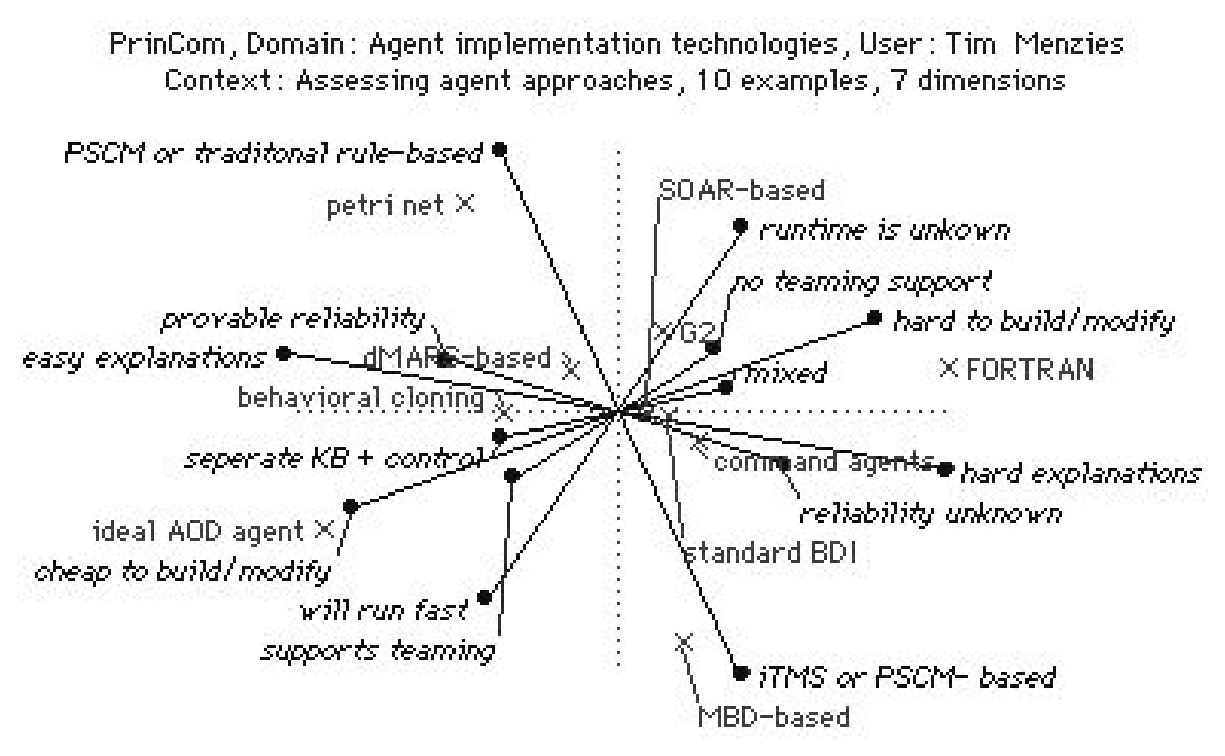
\includegraphics[width=5in]{star.eps}

{\em \begin{quote} {\sffamily This figure is generated from \protect\fig{table}
via a principle components analysis to grid the data. 2-D positions are
generated via first isolating combination of factors that are strongly
correlated. These factors define a transform space into which the various
technologies described in this article can be mapped into a 2-D space. This
diagram can be used to gain an intuitive view of what technologies are similar
(they appear closer together on this diagram).
 }\end{quote}}
  \end{center}
  \caption{Clusters of
agent technologies. Generated from the web-based repertory grid
server at \protect\url{http://gigi.cpsc.ucalgary.ca/} using the
dimensions of \fig{table}.}\label{fig:cluster}
\end{figure}

Apart from \fig{cluster}, we have also seen that different design
goals select different agent implementation technologies:
 \bi \item If the
goal is human cognitive modeling, then avoid low-level
representations. High-level representation schemes mentioned here
were SOAR and the BDI-based tools.
\item
If committed to intentionality, then use BDI-based tools such as
dMARS or the command agents extension.
\item If the goal is raw execution speed, use low-level representations
plus a fast theorem prover. Two such candidates are the decision
trees from behavioral cloning or  propositional encoding with the
iTMS.
\item
If the goal is explanation/justification of system behaviour, use
some technology that offers high level views of the system. Two
such systems reviewed here are the graphical interfaces of G2 or
systems that use high-level representations that match local
domain knowledge (e.g. command agents).
\item
If the goal is highly-reliable systems, then use petri nets.
\item If the goal is to model elaborate teaming interactions, then
hire AI specialists and conduct a research program to extend the
state-of-the-art in agent systems. \item If the goal is to reduce
maintenance costs, then consider automatically generating the
agent using behavioral cloning. Alternatively, if the goal is to
increase revenue through maintenance requests, then use FORTRAN.
\ei







\section*{Acknowledgements}The contents of this
paper were greatly enhanced by the lively discussion at the
Australian workshop on agent-oriented systems organized by Leon
Sterling (Melbourne University) and Simon Goss (AOD).  All views
expressed here are the authors and may not reflect the consensus
view of that workshop.

This research was partially conducted at West Virginia University
under NASA contract NCC2-0979. The work was sponsored by the NASA
Office of Safety and Mission Assurance under the Software
Assurance Research Program led by the NASA IV\&V Facility.
Reference herein to any specific commercial product, process, or
service by trade name, trademark, manufacturer, or otherwise, does
not constitute or imply its endorsement by the United States
Government.

\bibliographystyle{abbrv}
\bibliography{refs}

\end{document}
